\tikzstyle{block} = [rectangle, draw, fill=blue!20,
text width=30em, text centered, rounded corners, minimum height=4em]
\tikzstyle{line} = [draw, -latex']
\tikzstyle{cloud} = [draw, ellipse,fill=red!20, node distance=3cm,
minimum height=2em]

\chapter{Implementation}
\label{ch:implementation}
Section~\ref{sec:user-documentation} assists the end-users to use the system.
In Section~\ref{sec:project-presentation} we will take a look at the project structure.
Section~\ref{sec:configuration} describes how the project can be deployed and configured.
Section~\ref{sec:system-architecture} covers system architecture, namely the
communication protocols, frameworks, and APIs that are used in the system.
Finally, in Section~\ref{sec:technical-requirements-and-hardware}, we describe the technical
requirements and hardware used in the system.

%%%%%%%%%%%%%%%%%%%%%%%%%%%%%%%%%%%%%%%%%%%%%%%%%%%%%%%%%%%%%%%%%%%%%%%%%%%%%%%%%%%%%%%%%%%%%%%%%%%%%%%%%%%%%%%%%%%%%%%%
\section{User Documentation}
\label{sec:user-documentation}
When a user runs the android application for the first time, it displays the form that a
user has to fill in order to configure his phone.
For that, the user needs to follow the steps:

\begin{itemize}
    \item Choose the beacon ID that will help this application to measure the distance between devices.
    \item Give his mascot a custom name.
    \item Choose one out of five personalities displayed on the screen.
\end{itemize}

Figure~\ref{fig:MascotRegistrationUI} shows the user interface of the mascot application during the device registration.
\begin{figure}[hbt!]
    \centering
    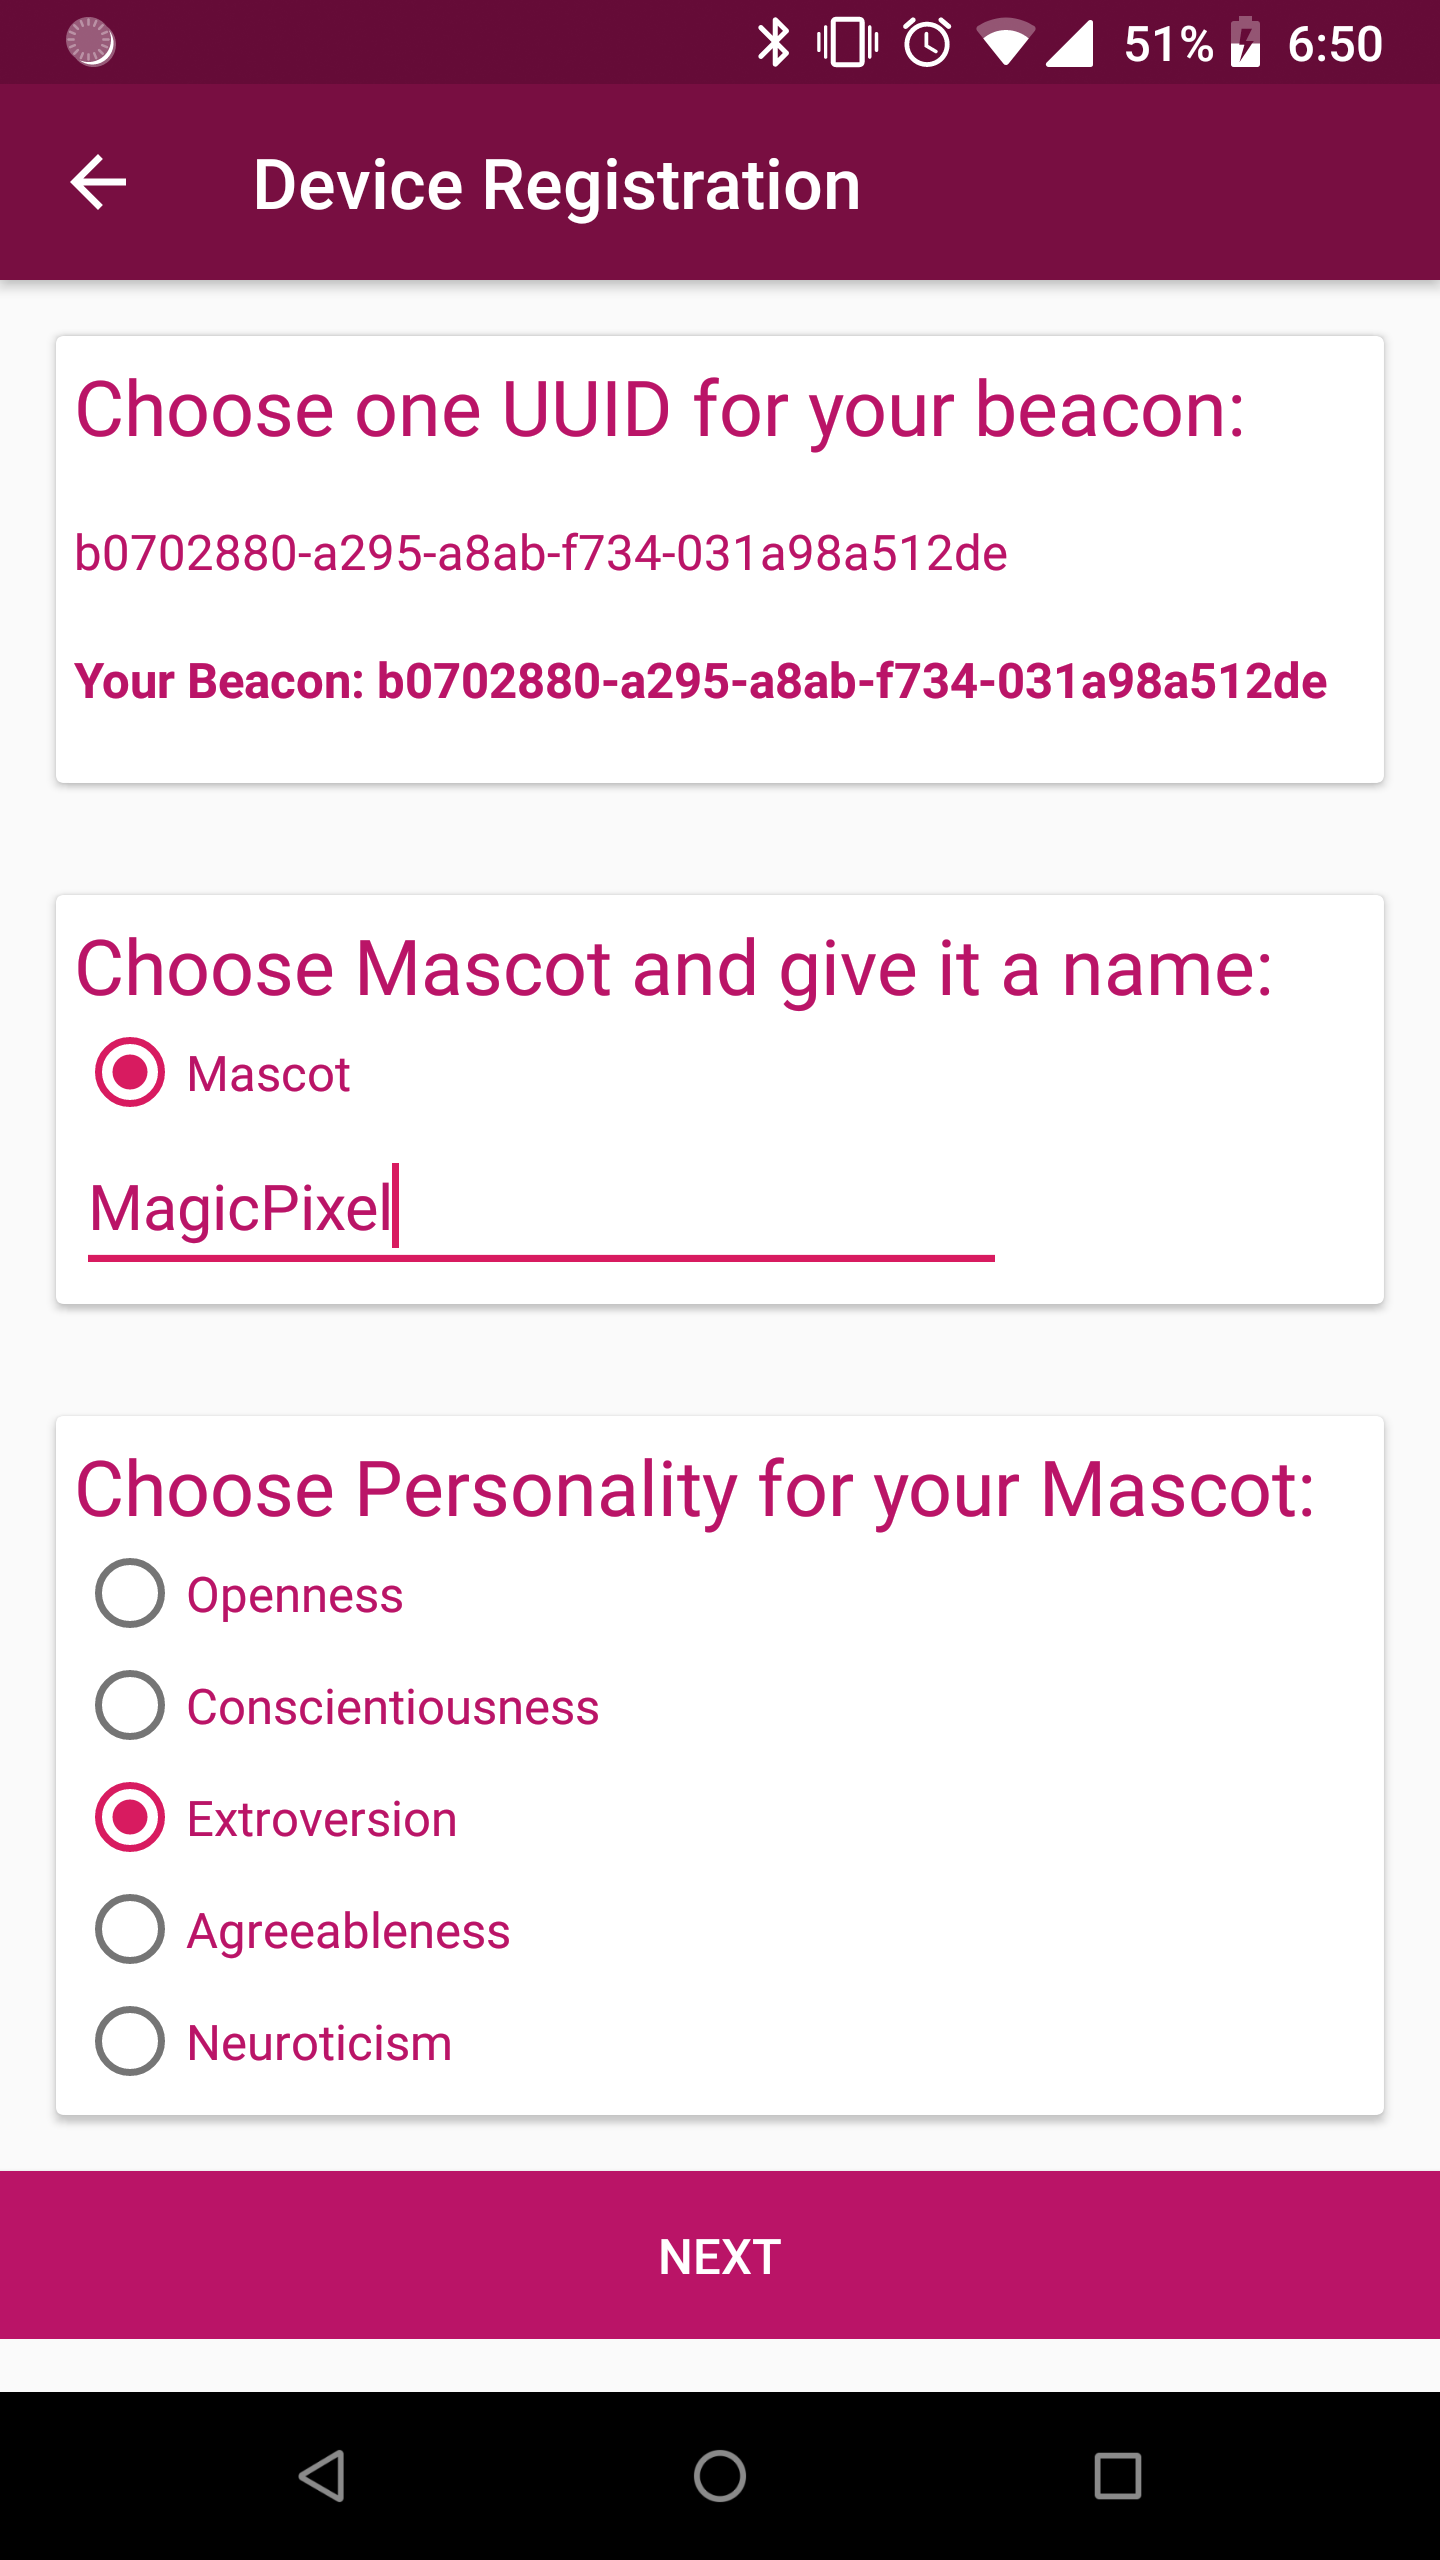
\includegraphics[scale=0.10]{MascotRegistrationUI.png}
    \caption{The screen capture of the user interface of the device registration page in mascot application.}
    \label{fig:MascotRegistrationUI}
\end{figure}

After pressing the next button, such information as beacon ID,
the type, name, and the personality of the device are sent to the server and saved in the database.
Starting from here, no further user interaction with the mobile phone is needed, the user can walk
around and approaching other devices such as other phones, lamps, speakers, and tablets.
The application starts to measure the distance to all other beacons according to the users'
movements and sends this information to a server.

%%%%%%%%%%%%%%%%%%%%%%%%%%%%%%%%%%%%%%%%%%%%%%%%%%%%%%%%%%%%%%%%%%%%%%%%%%%%%%%%%%%%%%%%%%%%%%%%%%%%%%%%%%%%%%%%%%%%%%%%
\section{Project Presentation}
\label{sec:project-presentation}
The project consists of the client-side with two Android applications for mascot i.e.\ phone and tablet.
The server is responsible for coordinating client applications.

The \texttt{AutonomousSystemThesis} consists of three directories:

\begin{itemize}
    \item \texttt{MyMascotApp}: The android application registers the phone in the system and measures the distance
    from the phone and to all beacon tags located in the room.
    \item \texttt{MyTabletApp}: The android application that is registering the tablet in the system and displaying colors according to the personality of approaching mascot
    \item \texttt{server}: allows the management of all devices and beacons, and the coordination of all client applications.
\end{itemize}

The project structure is demonstrated in Figure~\ref{lst:library-structure}.

\begin{figure}[!htbp]
    \definecolor{folderbg}{RGB}{124, 166, 198}
    \definecolor{folderborder}{RGB}{110, 144, 169}

    \def\Size{4pt}
    \tikzset{
    folder/.pic={
    \filldraw[draw=folderborder, top color=folderbg!50, bottom color=folderbg]
    (-1.05*\Size, 0.2\Size+5pt) rectangle ++(.75*\Size, -0.2\Size-5pt);
    \filldraw[draw=folderborder, top color=folderbg!50, bottom color=folderbg]
    (-1.15*\Size, -\Size) rectangle (1.15*\Size, \Size);
    },
    file/.pic={
    \filldraw[draw=folderborder, top color=folderbg!5, bottom color=folderbg!10]
    (-\Size, .4*\Size+5pt) coordinate(a) |- (\Size, -1.2*\Size) coordinate(b) -- ++(0, 1.6*\Size) coordinate(c) -- ++(-5pt, 5pt) coordinate(d) -- cycle(d) |- (c);
    },
    }

    \centering
    \begin{forest}
        for tree={
        font=\ttfamily,
        grow'=0,
        child anchor=west,
        parent anchor=south,
        anchor=west,
        calign=first,
        inner xsep=8pt,
        edge path={
        \noexpand\path [draw, \forestoption{edge}]
        (!u.south west) +(7.5pt,0) |- (.child anchor) pic {folder} \forestoption{edge label};
        },
        file/.style={
        edge path={
        \noexpand\path [draw, \forestoption{edge}]
        (!u.south west) +(7.5pt, 0) |- (.child anchor) pic {file} \forestoption{edge label};
        },
        },
        before typesetting nodes={
        if n=1
        {insert before={[,phantom]}}
        {},
        },
        fit=band,
        before computing xy={l=15pt},
        }
        [
        [AutonomousSystemThesis
        [MyMascotApp, label=right:- Android application for mascot
        ]
        [MyTabletApp, label=right:- Android application for tablet
        ]
        [server, label=right:- Server application for devices management
        ]
        ]
        ]
    \end{forest}

    \caption{The folder structure of the whole system}
    \label{lst:library-structure}
\end{figure}
%%%%%%%%%%%%%%%%%%%%%%%%%%%%%%%%%%%%%%%%%%%%%%%%%%%%%%%%%%%%%%%%%%%%%%%%%%%%%%%%%%%%%%%%%%%%%%%%%%%%%%%%%%%%%%%%%%%%%%%%

\section{System Architecture}
\label{sec:system-architecture}
For multi-device support used centralized architecture, where all devices inform the server about their state in real-time.
Subsequently, the server changes the states of all other devices accordingly.
Moreover, the centralized system has a simpler design that excludes any consensus problem.
All devices communicate with each other through the server that makes decisions.

\subsection{Module descriptions}
\label{subsec:module-descriptions}
\textbf{\texttt{MyMascotApp}} is an Android application that has the following responsibilities:
\begin{itemize}
    \item The application registers the phone in the system, namely the ID of a beacon that it is attached,
    mascot custom name, and the personality of a mascot.
    \item The application measures the distance from the device-phone to all other beacons in the system.
    \item The application vibrates the phone with the vibration duration that the server sent to it.
\end{itemize}

%%%%%%%%%%%%%%%%%%%%%%%%%%%%%%%%%%%%%%%%%%%%%%%%%%%%%%%%%%
\textbf{\texttt{MyTabletApp}} is an Android application that has the following functionalities:
\begin{itemize}
    \item The application registers the tablet in the system, namely ID of a beacon that it is attached to it.
    \item Every second, the tablet application polls data from the server, where as a response it gets specific color code.
    \item The application changes the background color of a screen to a color that is retrieved from the server.
\end{itemize}

%%%%%%%%%%%%%%%%%%%%%%%%%%%%%%%%%%%%%%%%%%%%%%%%%%%%%%%%%%
\textbf{\texttt{server}} is a server application that has the following features:
\begin{itemize}
    \item Manages a database that consists of three tables (devices, distances, and personality).
    \item Implements controllers that handle the client requests such as post requests of device registration,
    distances, and get requests of required data from the database.
    \item Server checks whether the distance of all devices falls into the predefined distance range of the Proxemics theory.
    \item When the user reaches the lamp, the server requests Philips Hue API to change color based on the personality retrieved from the database.
    \item When the user approaches speakers, play audio files concurrently using the Audio File Play
    utility or \texttt{afplay}.
\end{itemize}

The folder structure of the server application is demonstrated in Figure~\ref{lst:library-structure-server}.

\begin{figure}[hbt!]
    \definecolor{folderbg}{RGB}{124, 166, 198}
    \definecolor{folderborder}{RGB}{110, 144, 169}

    \def\Size{4pt}
    \tikzset{
    folder/.pic={
    \filldraw[draw=folderborder, top color=folderbg!50, bottom color=folderbg]
    (-1.05*\Size, 0.2\Size+5pt) rectangle ++(.75*\Size, -0.2\Size-5pt);
    \filldraw[draw=folderborder, top color=folderbg!50, bottom color=folderbg]
    (-1.15*\Size, -\Size) rectangle (1.15*\Size, \Size);
    },
    file/.pic={
    \filldraw[draw=folderborder, top color=folderbg!5, bottom color=folderbg!10]
    (-\Size, .4*\Size+5pt) coordinate(a) |- (\Size, -1.2*\Size) coordinate(b) -- ++(0, 1.6*\Size) coordinate(c) -- ++(-5pt, 5pt) coordinate(d) -- cycle(d) |- (c);
    },
    }

    \centering
    \begin{forest}
        for tree={
        font=\ttfamily,
        grow'=0,
        child anchor=west,
        parent anchor=south,
        anchor=west,
        calign=first,
        inner xsep=8pt,
        edge path={
        \noexpand\path [draw, \forestoption{edge}]
        (!u.south west) +(7.5pt,0) |- (.child anchor) pic {folder} \forestoption{edge label};
        },
        file/.style={
        edge path={
        \noexpand\path [draw, \forestoption{edge}]
        (!u.south west) +(7.5pt, 0) |- (.child anchor) pic {file} \forestoption{edge label};
        },
        },
        before typesetting nodes={
        if n=1
        {insert before={[,phantom]}}
        {},
        },
        fit=band,
        before computing xy={l=15pt},
        }
        [
        [Server
        [controller, label=right:- Responsible for handling the client requests.
        ]
        [database, label=right:- Database models and table definitions.
        ]
        [ServerApplication.java, file, label=right:- The entry point to the server application.
        ]
        ]
        ]
    \end{forest}

    \caption{The folder structure of the server application}
    \label{lst:library-structure-server}
\end{figure}
%%%%%%%%%%%%%%%%%%%%%%%%%%%%%%%%%%%%%%%%%%%%%%%%%%%%%%%%%%%%%%%%%%%%%%%%%%%%%%%%%%%%%%%%%%%%%%%%%%%%%%%%%%%%%%%%%%%%%%%%

\subsection{Software stack and protocols}
\label{subsec:software-stacks}

The following programming languages, frameworks, and APIs were used to implement the system.

For client applications:
\begin{itemize}
    \item Android framework with Java language.
    \begin{itemize}
        \item NSD API - Network Service Discovery.
    \end{itemize}
    \item AltBeacon Library.
\end{itemize}

For the server-side:
\begin{itemize}
    \item Spring Framework with Java language.
    \item DNS-SD\@.
    \item Philips Hue API\@.
    \item Music Playback component.
\end{itemize}

%%%%%%%%%%%%%%%%%%%%%%%%%%%%%%%%%%%%%%%%%%%%%%%%%%%%%%%%%%%%%%%%%%%%%%%%%%%%%%%%%%%%%%%%%%%%%%%%%%%%%%%%%%%%%%%%%%%%%%%%
\subsection{Database and server}
\label{subsec:database-and-server}
Network requests are handled by controllers using the Spring framework on the server-side.
It also allows easy data access to simply connecting and working with the database.

For database management, we use an open-source relational database system known as PostgreSQL\@.

Database schema and models are defined using Hibernate - an ORM (object relation mapping) framework.
Hibernate is also responsible for managing database tables in PostgreSQL\@.
For the detailed instructions on how to set up the database and run the server
see Appendix~\ref{sec:setting-up-the-server.}-~\ref{sec:starting-the-server.}.
%%%%%%%%%%%%%%%%%%%%%%%%%%%%%%%%%%%%%%%%%%%%%%%%%%%%%%%%%%%%%%%%%%%%%%%%%%%%%%%%%%%%%%%%%%%%%%%%%%%%%%%%%%%%%%%%%%%%%%%%

\subsection{Service discovery}
\label{subsec:service-discovery.}
The way android clients discover a server is by using mDNS implementation on Android called NSD API\@.

\textbf{NSD API} (Network Service Discovery) is an Android implementation of Multicast DNS\@.
In order to make requests the Android applications need to know the IP address and port of services.
NSD API helps the client to discover the server.
\texttt{NSDHelper.java} module allows the client-applications to find an HTTP server in the local network that supports
services that clients are interested in.
In our case, we specified \_socialiot.\_tcp type of service.

\textbf{DNS-SD} is an implementation of mDNS protocol on macOS\@.
In this project, it is used to register and publish the server information, such as the port number and the service name.
Here is an example of how it can be used to set up the \texttt{AutonamousThesisProject}:
\begin{lstlisting}
    @\textcolor{green!40!black}{dns-sd -R mythesis \_socialiot.\_tcp local 8080}@
\end{lstlisting}
In the command specified above, \textbf{\emph{mythesis}} is a service name;
\textbf{\emph{\_socialiot.\_tcp}} is a service type;
\textbf{\emph{8080}} is a port number with domain type \textbf{\emph{local}}.
The parameter \_socialiot.\_tcp must match, since the client applications using NSD API
will start looking for this specific service type.

%%%%%%%%%%%%%%%%%%%%%%%%%%%%%%%%%%%%%%%%%%%%%%%%%%%%%%%%%%%%%%%%%%%%%%%%%%%%%%%%%%%%%%%%%%%%%%%%%%%%%%%%%%%%%%%%%%%%%%%%
\subsection{Registering devices in the system}
\label{subsec:registering-devices-in-the-system.}
Every user can register its mascot in the system by running \texttt{MyMascotApp} and following the instructions on the screen.
The detailed description of how to configure the smartphone for the mascot application is given in
Section~\ref{sec:user-documentation}.

The registration of such devices as the tablet, the lamp, and the speakers must be performed
by the developers using \texttt{MyTabletApp}.
So, the tablet application is the device that registers all social devices with a fixed location.
Also, the tablet application registers in the system all five personality traits with their
associated actions such as color, music type, and the vibration level.
The registration of all devices and the personality traits can be performed by following the instructions on the screen.
Figure~\ref{fig:PersInit} is the screenshot of the tablet application that shows the information of the data that will
be sent to the server about the personality traits and associated actions.

You can also find the step-by-step instructions on how to run both the mascot and the tablet applications in
Appendix~\ref{sec:setting-up-the-client-applications.}.

\begin{figure}[hbt!]
    \centering
    \begin{subfigure}{.40\textwidth}
        \centering
        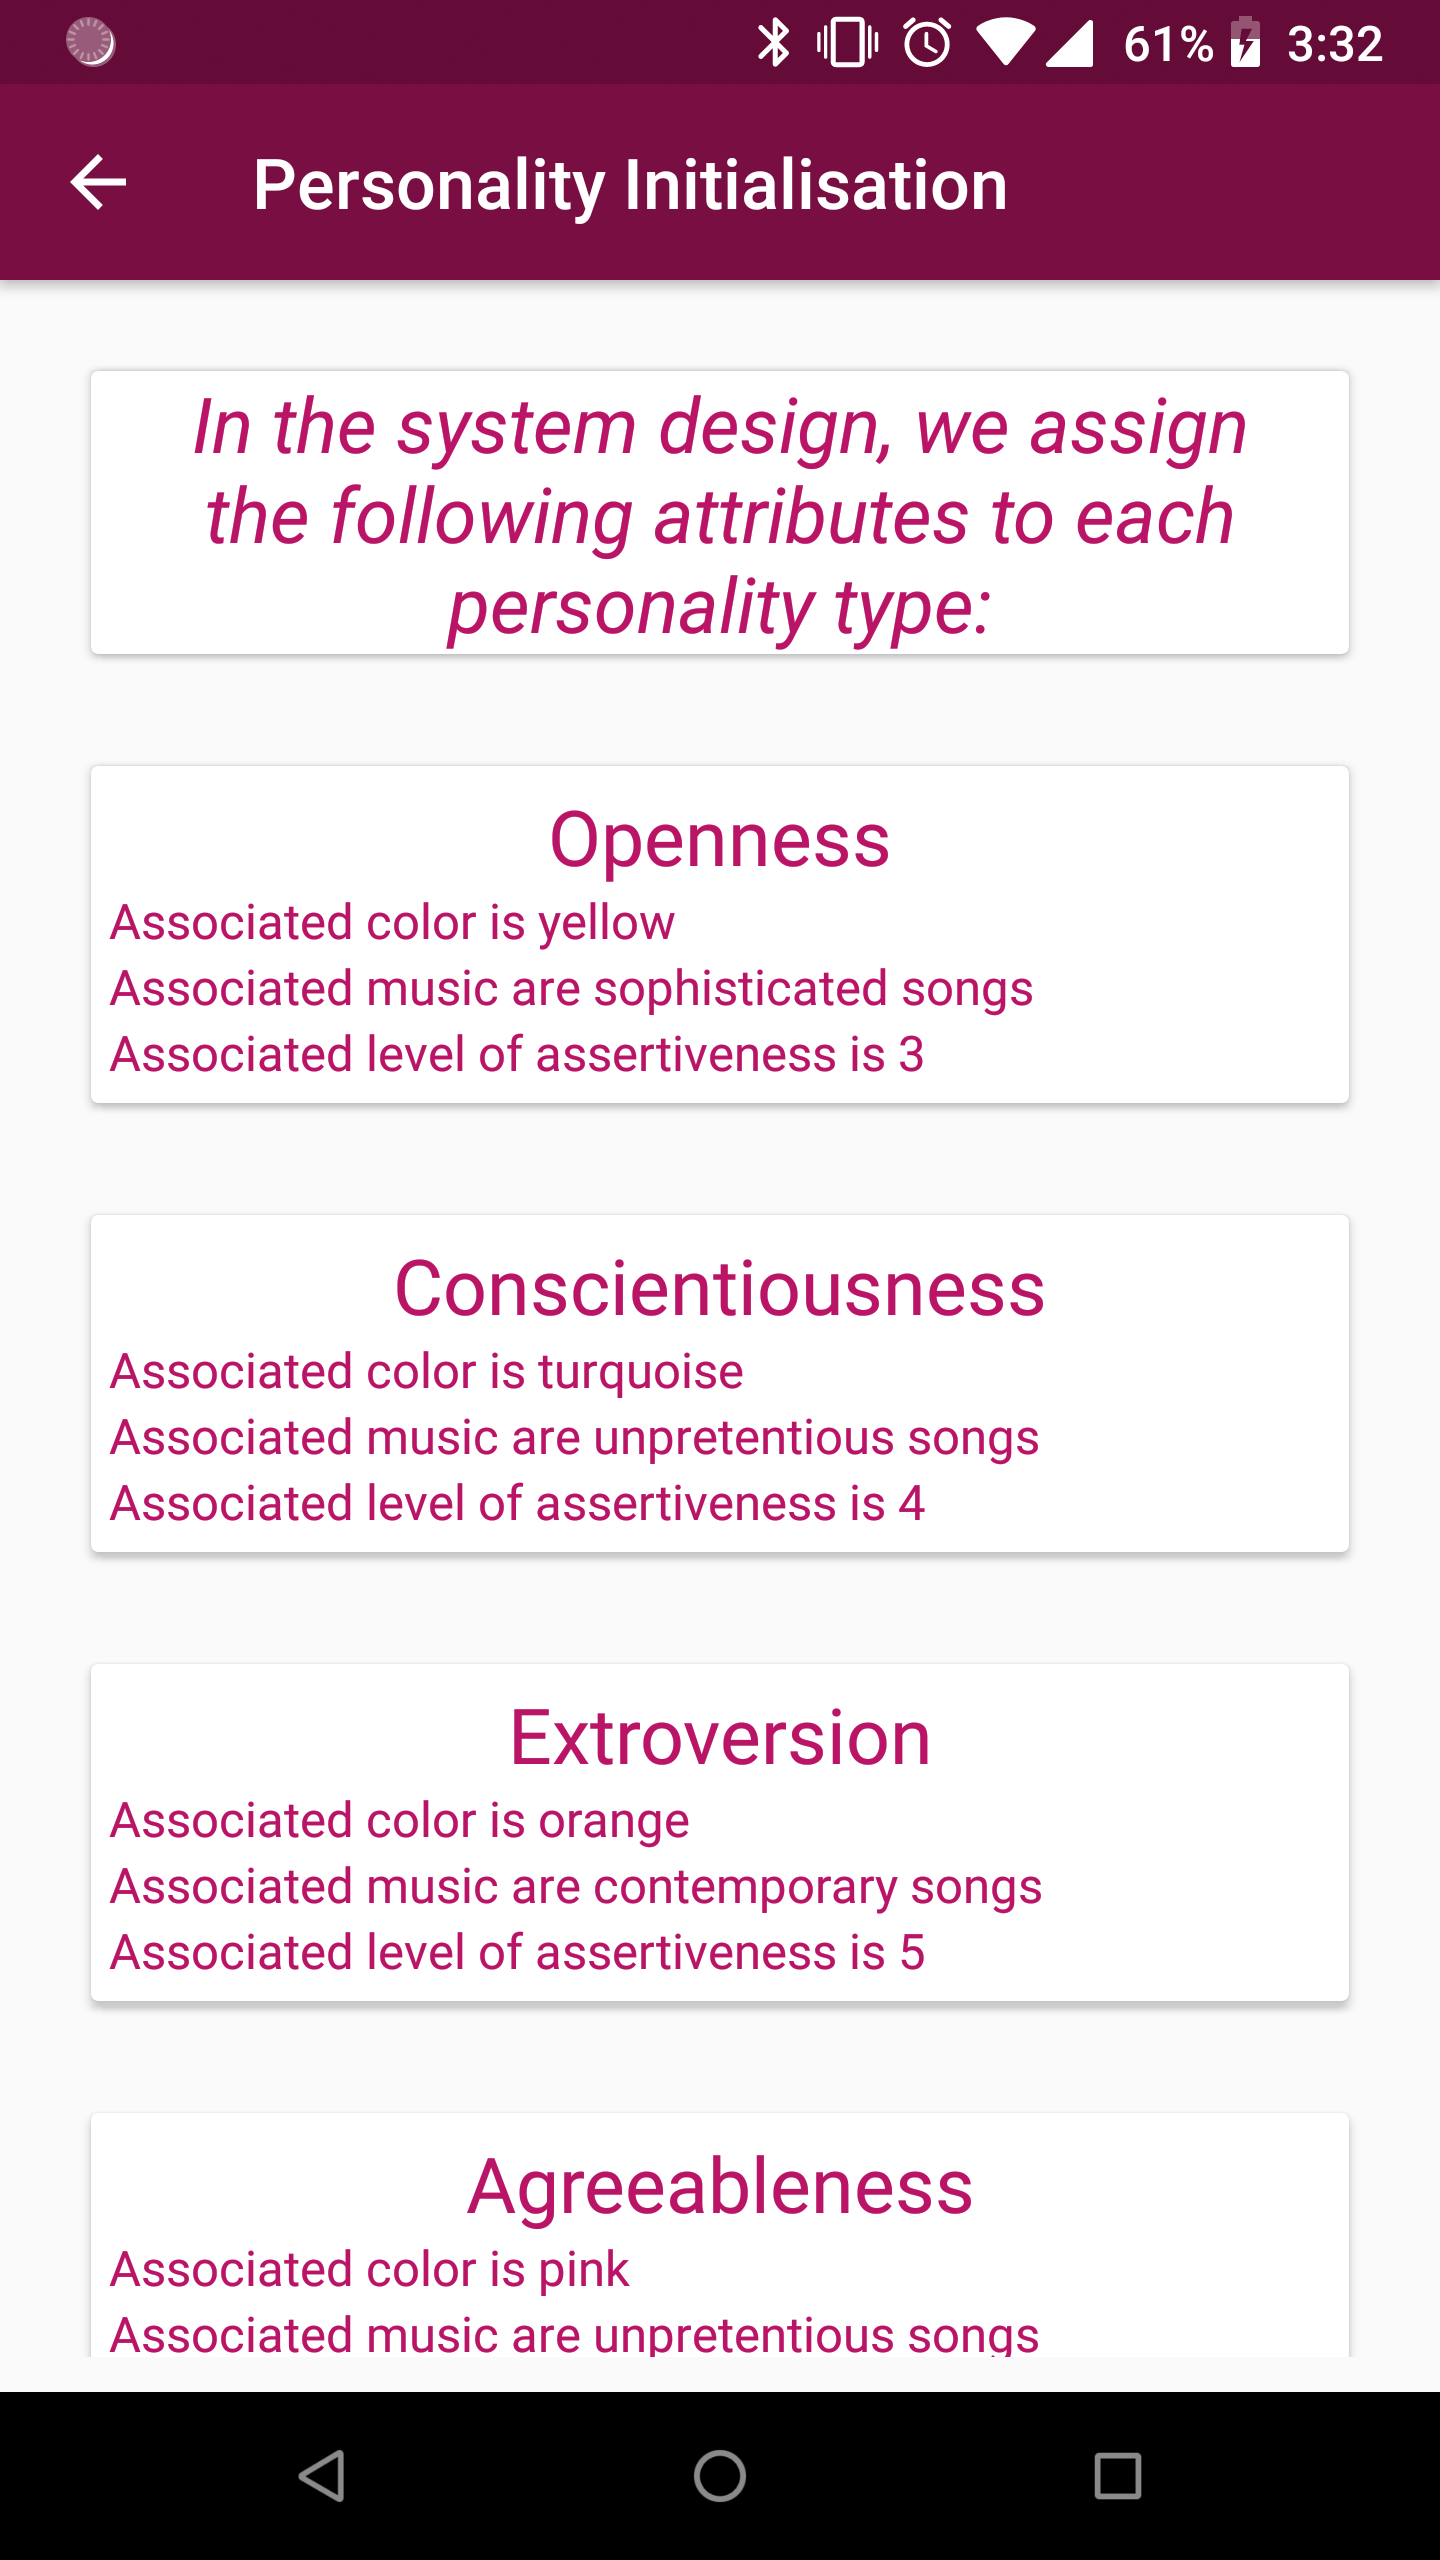
\includegraphics[width=1\linewidth]{PersInit1.png}
        \caption{The top of the page.}
        \label{fig:sub1}
    \end{subfigure}\hfill%
    \begin{subfigure}{.40\textwidth}
        \centering
        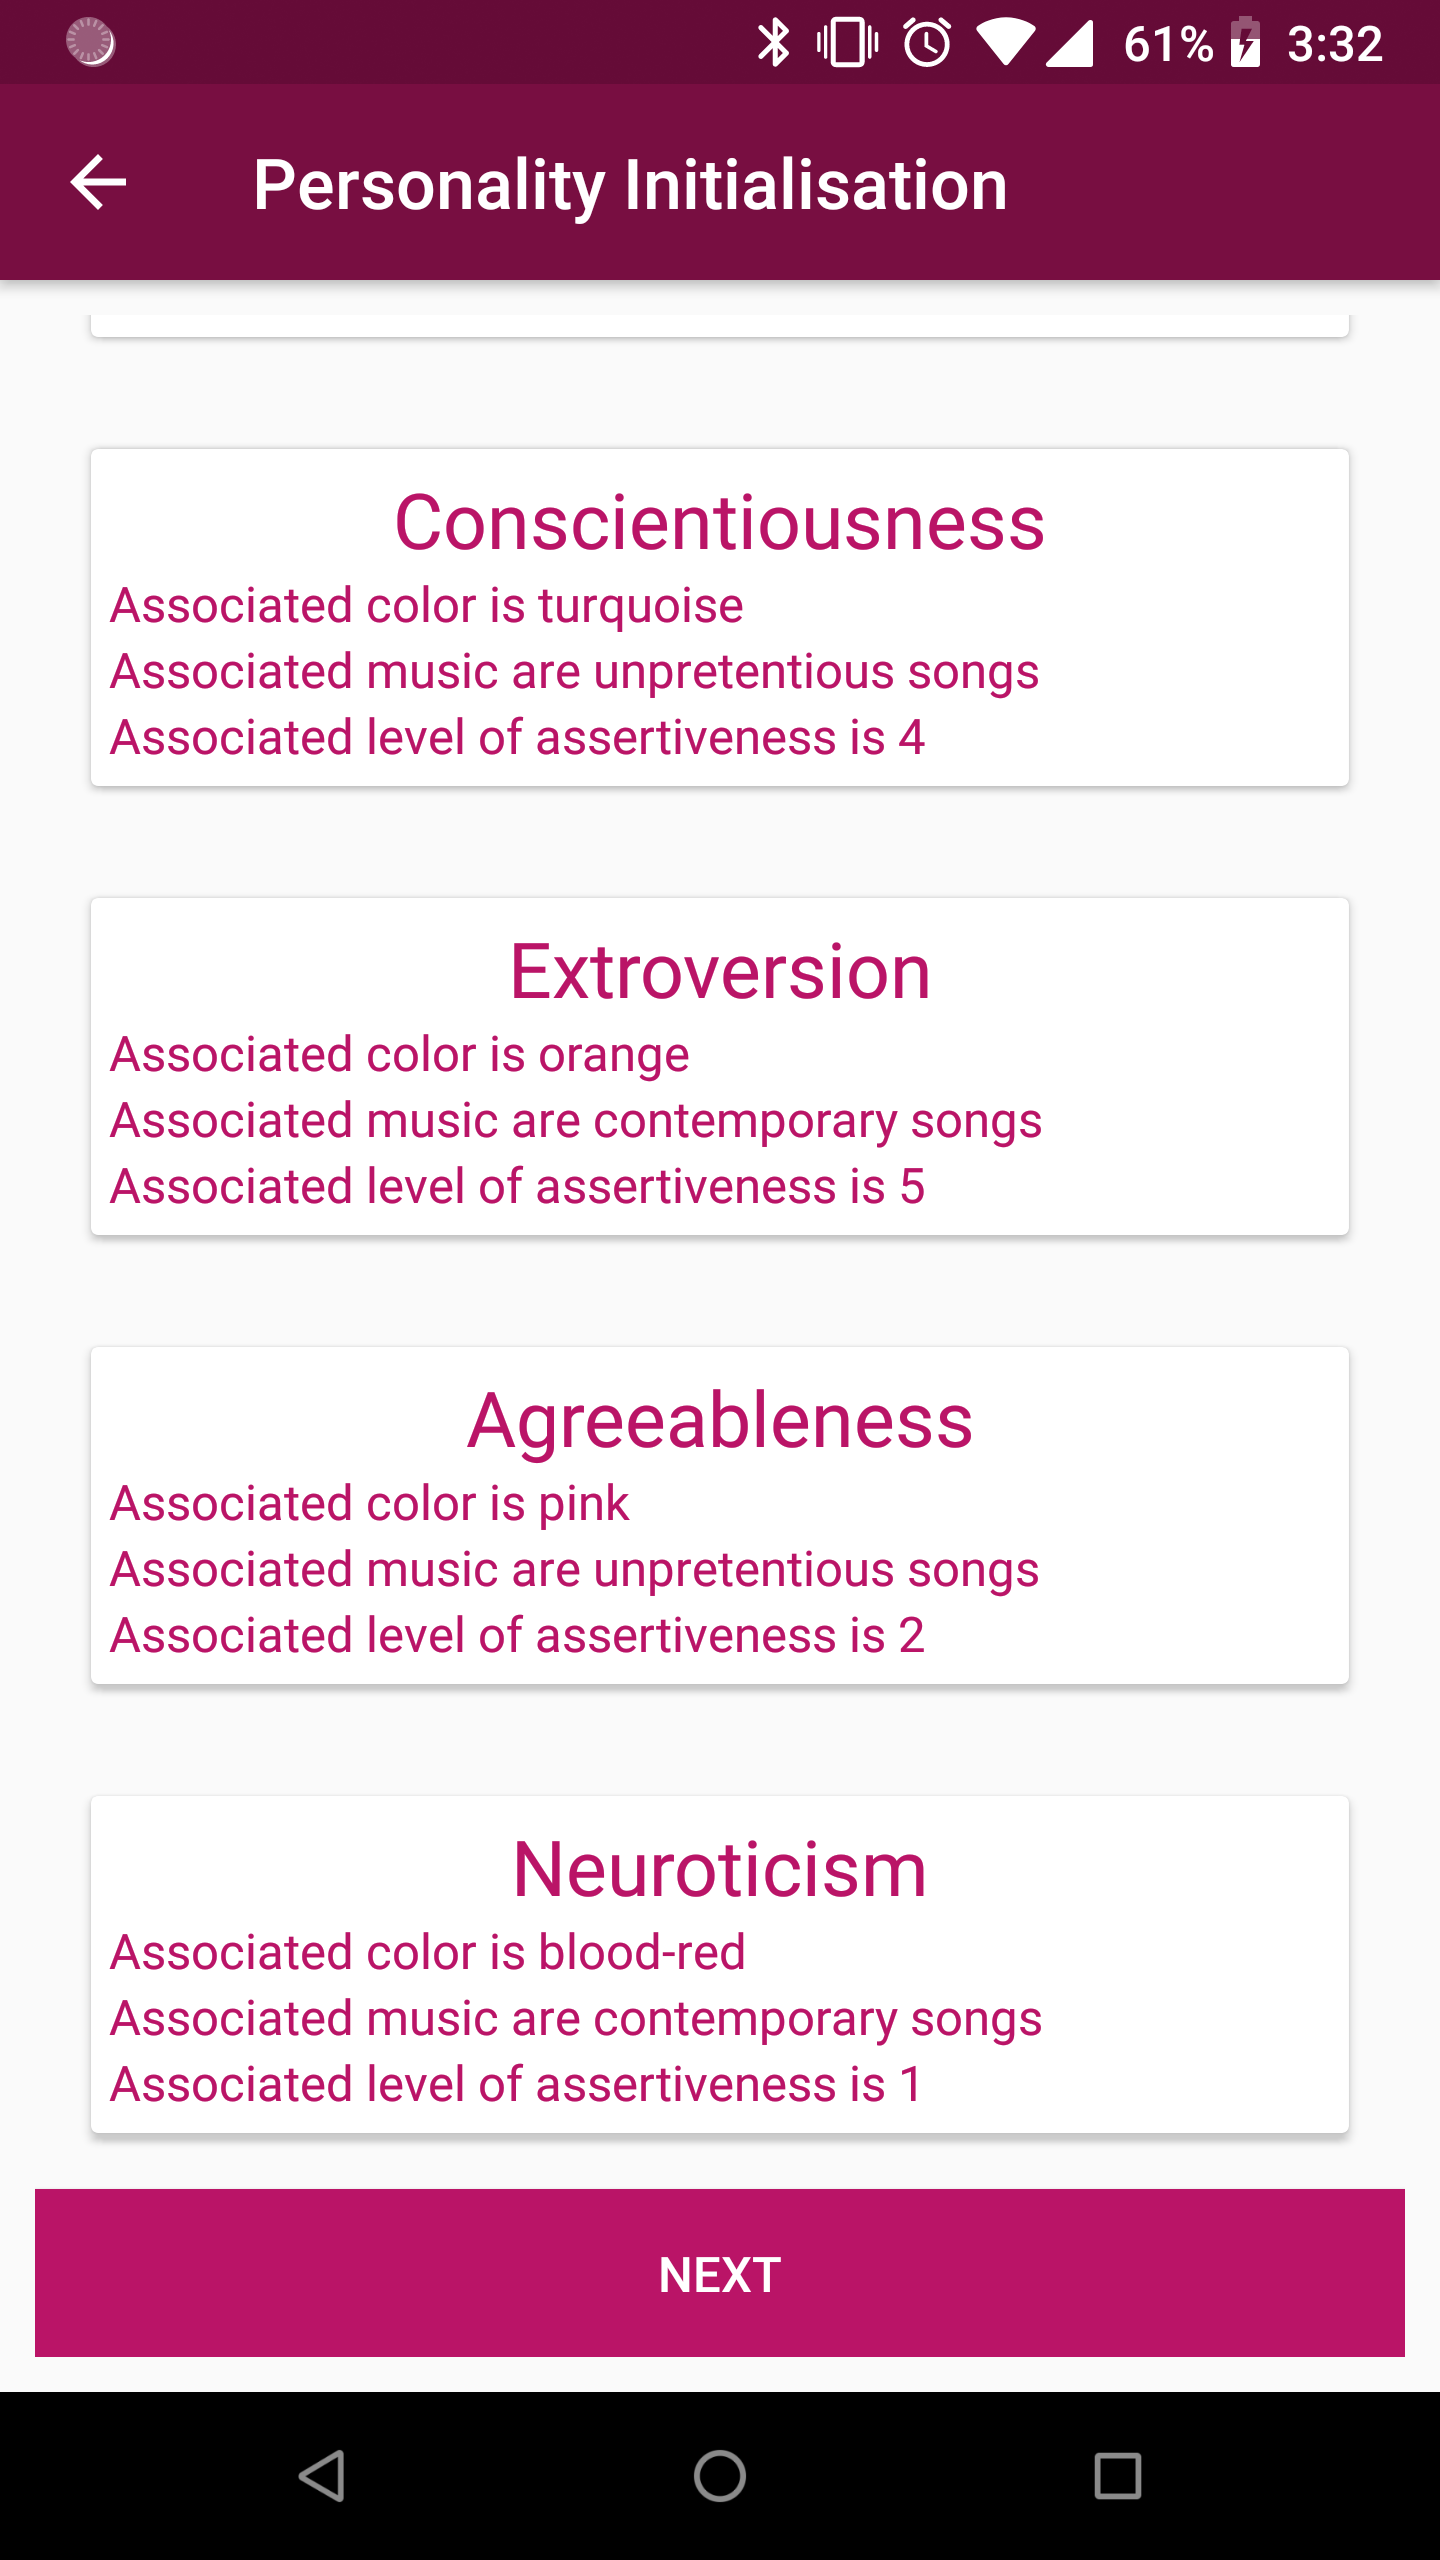
\includegraphics[width=1\linewidth]{PersInit2.png}
        \caption{The bottom of the page.}
        \label{fig:sub2}
    \end{subfigure}\hfill
    \caption{The screen capture of the user interface of the personality registration in tablet application.}
    \label{fig:PersInit}
\end{figure}

%%%%%%%%%%%%%%%%%%%%%%%%%%%%%%%%%%%%%%%%%%%%%%%%%%%%%%%%%%%%%%%%%%%%%%%%%%%%%%%%%%%%%%%%%%%%%%%%%%%%%%%%%%%%%%%%%%%%%%%%
\subsection{Measuring distance between devices}
\label{subsec:measuring-distance-between-devices.}
\textbf{AltBeacon Library} is a library that provides APIs to interact with beacon tags.
Beacon tags are broadcast-only Bluetooth Low Energy (BLE) radio transmitters which communicate by
transmitting their proximity to the Android applications that supports BLE technology.
With the help of AltBeacon Library, \texttt{MyMascotApp} detects beacon tags nearby
and uses this information to measure the distance.
The accuracy precision that \texttt{MyMascotApp} can measure the distance is around a half meter
with a ten-second margin for new positions.

\subsection{The communication between two mascots}
\label{subsec:the-communication-between-two-mascots.}
The communication between devices and the workflow of the system is described in Figure~\ref{fig:Workflow}.
The figure describes the interaction between two phones and step by step including requests
that clients and a server send each other.

After the client application finds the server in a local network, it looks for all nearby beacon tags.
When the user types the custom name for his mascot, the personality, and the beacon, the client
application registers all this information in the system.
The client application starts to measure the distance to all beacon tags that are located near other devices.
The distance information is constantly sent to the server, where as soon as mascot approaches the other mascot within
45 cm, the server retrieves the personality information of approaching mascot with the associated vibration duration
from a database.
Afterward, the server passes the vibration information to the client, which in turn triggers the
phone to vibrate with an invoked vibration level.

\tikzstyle{startstop} = [rectangle, minimum width=3cm, minimum height=1cm,
text width=8cm, text centered, draw=black, fill=orange!30]
\tikzstyle{process} = [rectangle, minimum width=3cm, minimum height=1cm,
text width=8cm, text centered, draw=black, fill=orange!30]
\tikzstyle{io} = [trapezium, trapezium left angle=70, trapezium right angle=110, minimum width=3cm, minimum height=1cm,
text width=4.5cm, text centered, draw=black, fill=blue!30]
\tikzstyle{decision} = [diamond, minimum width=1cm, minimum height=0.5cm, aspect=3.5,
text width=5cm, text centered, draw=black, fill=green!30]
\tikzstyle{arrow} = [thick,->,>=stealth]
\begin{figure}[hbt!]
    \centering
    \begin{tikzpicture}[node distance=1.7cm]
        \node (start) [startstop] {Client searches for a server using NSD API};
        \node (pro) [process, below of=start] {Client looks for beacon tags using AltBeacon Library};
        \node (in1) [io, below of=pro] {Client registers device};
        \node (pro1) [process, below of=in1] {Client sends requests to the server to check if the device is registered};
        \node (dec1) [decision, below of=pro1, yshift=-0.5cm] {Server checks if the device is in database};
        \node (pro2) [process, below of=dec1, yshift=-0.5cm] {Client starts measuring the distance to all beacon tags};
        \node (pro3) [process, below of=pro2] {Client sends distance information to server};
        \node (dec2) [decision, below of=pro3, yshift=-0.5cm] {Server checks distance between both mascots < 45cm};
        \node (pro4) [process, below of=dec2, yshift=-0.5cm] {Client gets vibration level from server};
        \node (pro5) [process, below of=pro4] {Client triggers vibration with specific duration};
        \draw [arrow] (start) -- (pro);
        \draw [arrow] (pro) -- (in1);
        \draw [arrow] (in1) -- (pro1);
        \draw [arrow] (pro1) -- (dec1);
        \draw [arrow] (dec1.east) -- ++(2em,0) node[above] {no} -- ++(2em,0) |- (in1.east);
        \draw [arrow] (dec1) -- node[anchor=east] {yes} (pro2);
        \draw [arrow] (pro2) -- (pro3);
        \draw [arrow] (pro3) -- (dec2);
        \draw [arrow] (dec2.east) -- ++(2em,0) node[above] {no} -- ++(2em,0) |- (pro2.east);
        \draw [arrow] (dec2) -- node[anchor=east] {yes} (pro4);
        \draw [arrow] (pro4) -- (pro5);
    \end{tikzpicture}
    \caption{The interaction between two phones and a server with the libraries and APIs that it is using.}
    \label{fig:Workflow}
\end{figure}

\subsection{Working with lights}
\label{subsec:working-with-lights.}
The interaction between mascot and lamp happens using Philips Hue API\@.

\textbf{Philips Hue API} helps the server to control the hue system.
The workflow of the mascot-lamp interaction is similar to the mascot-mascot interaction (see Figure~\ref{fig:Workflow})
and all other interaction types.
The client measures the distance from the Android application to all beacons
in the system and constantly sends this information to the server.
The only difference is the use of Philips Hue API\@.
When the server encounters that the distance between mascot and lamp fits the Proxemics theory i.e.\ x<45, it
retrieves such parameters as hue, brightness, and saturation from the database and sends them
to the Hue bridge through Philips Hue API\@.
With the help of API, it can directly input commands such as changing light color which in turn will trigger the lamp to
change its lighting color.
All Philips Hue lamps need to be connected to the Philips Hue Bridge via an open
standards protocol called ZigBee Light Link which in turn helps devices to communicate with each other via the internet.
Figure~\ref{fig:InteractionMl} shows the visual representation of the mascot interacting with the lamp.

The important note for the implementation part is that all devices such as Philips Hue Bridge, server,
phones, and tablet have to be connected to the same network.
\begin{figure}[hbt!]
    \centering
    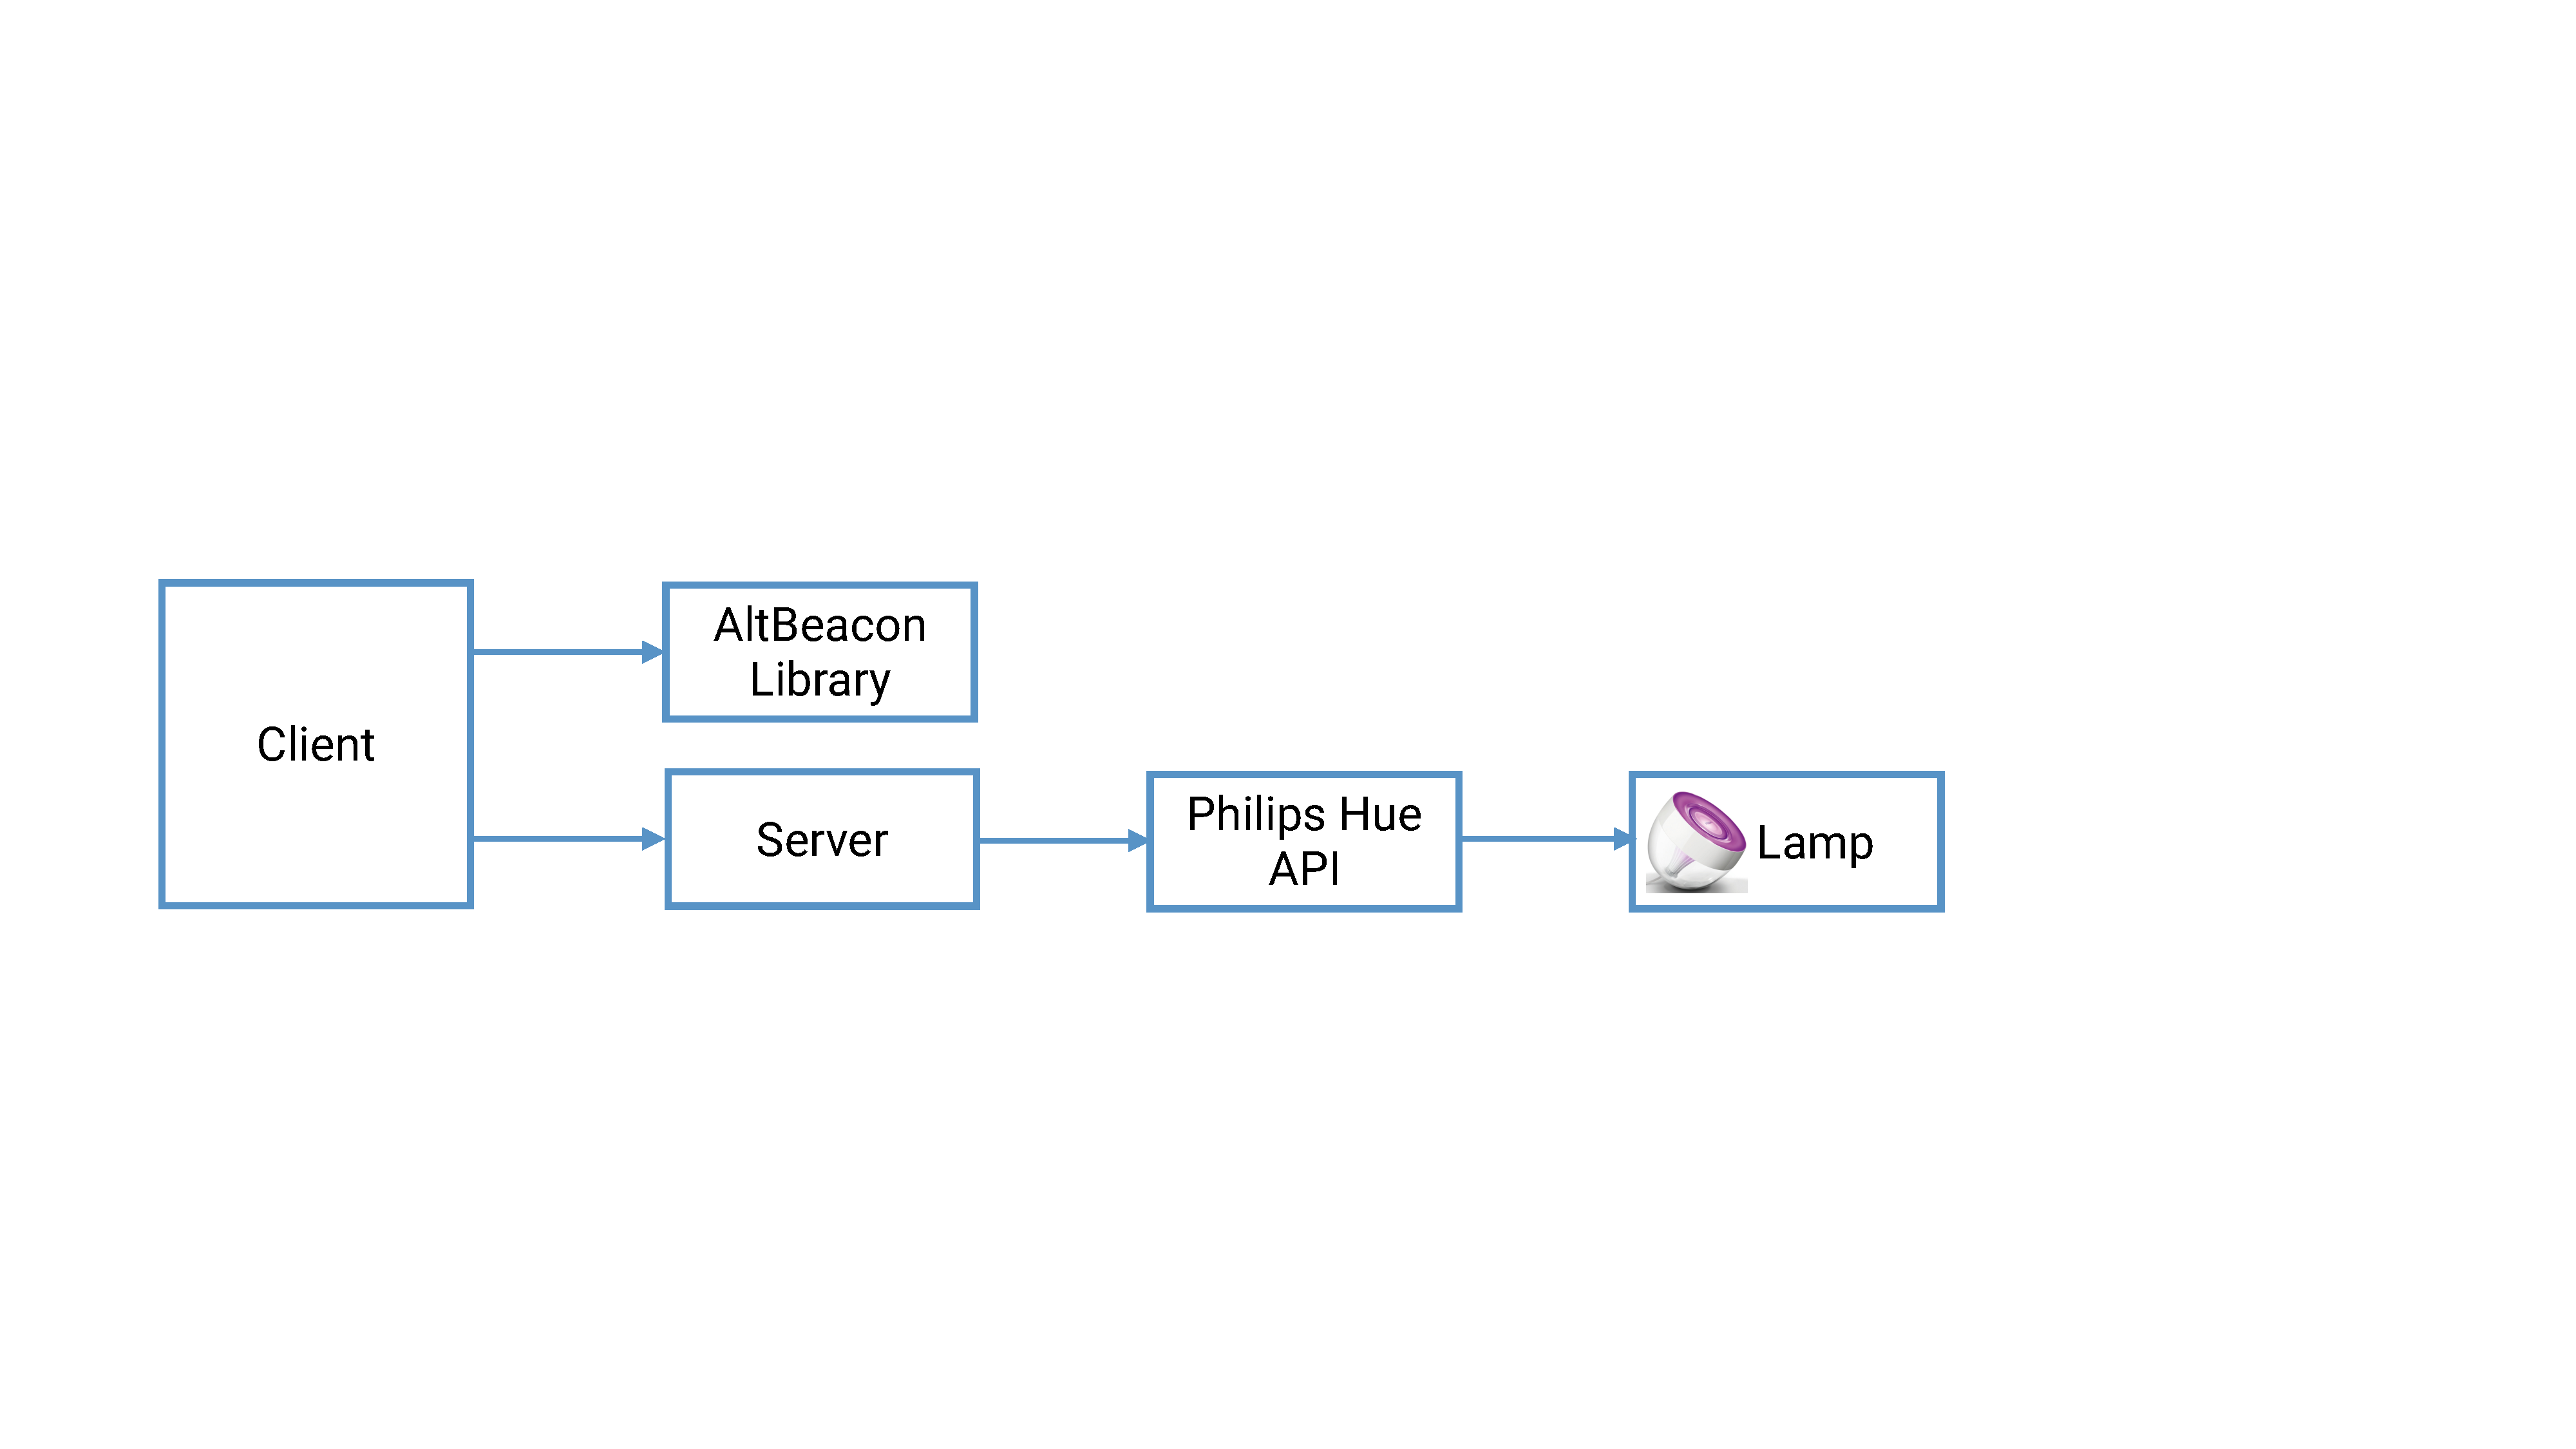
\includegraphics[scale=0.28]{InteractionM-L.pdf}
    \caption{Visual representation of mascot-lamp interaction.}
    \label{fig:InteractionMl}
\end{figure}

\section{Technical Requirements and Hardware}
\label{sec:technical-requirements-and-hardware}
The system comprises of the following devices: the phone with an attached beacon tag,
the lamp with a beacon tag, the tablet with a beacon tag, and speakers with a beacon tag.
Using the beacon tags that are located right next to devices, Android applications
measure the distance from themselves to all other devices.

Additionally, the following prerequisites have to be met:
\begin{itemize}
    \item Philips Hue lamps to be connected to the local network.
    \item The android application with the location and the Bluetooth permissions granted.
    \item The android application the operating system in order to use Bluetooth BLE must be higher than 6+.
    \item The server must be running on macOS to use \texttt{afplay} utility.
\end{itemize}
%%%%%%%%%%%%%%%%%%%%%%%%%%%%%%%%%%%%%%%%%%%%%%%%%%%%%%%%%%%%%%%%%%%%%%%%%%%%%%%%%%%%%%%%%%%%%%%%%%%%%%%%%%%%%%%%%%%%%%%%

\section{Configuration}
\label{sec:configuration}
The \texttt{AutonomousSystemThesis} can be configured in the following way:

To run the server, we pass the following arguments in the terminal:
\begin{lstlisting}
    @\textcolor{green!40!black}{mvn spring-boot:run -e -X -Dspring-boot.run.arguments=--hueUsername=<hue\_username>,--hueIPAddress=<hue\_ip\_address>,--musicFolderPath=<music\_folder\_path>}@
\end{lstlisting}

The Spring Boot Maven Plugin is used to run spring boot applications and generate build information.

Here, \emph{<hue\_ip\_address>} is an IP address assigned to our Philips Hue bridge.
Since you will have your smart lamps, you need to discover the IP address of your bridge.
The quickest way to discover it is to visit this website \footnote{\url{https://discovery.meethue.com}} which
will display the internal IP address of your bridge.
The username can be obtained by visiting the following website:

\url{https://<bridge IP address>/debug/clip.html}

where \emph{<bridge ip address>} is the internal IP address of your bridge.
The step-by-step instructions on how to get username and IP address of the Philips Hue bridge is described in
Appendix~\ref{sec:setting-up-the-philips-hue-bridge.}.
The more detailed guideline on how to discover the IP address and username of your bridge you can
find in the official Philips Hue Documentation\footnote{\url{https://developers.meethue.com/develop/get-started-2/}}.

The \emph{<music\_folder\_path>} is the path to all songs played when mascot approaches the speakers.
This path can be configurable and depends on where the project is saved.

The fully documented configuration of the database, server, and client applications are described in
Appendix~\ref{ch:the-instructions-of-the-system.}.

%\begin{figure}[H]
%    \centering
%    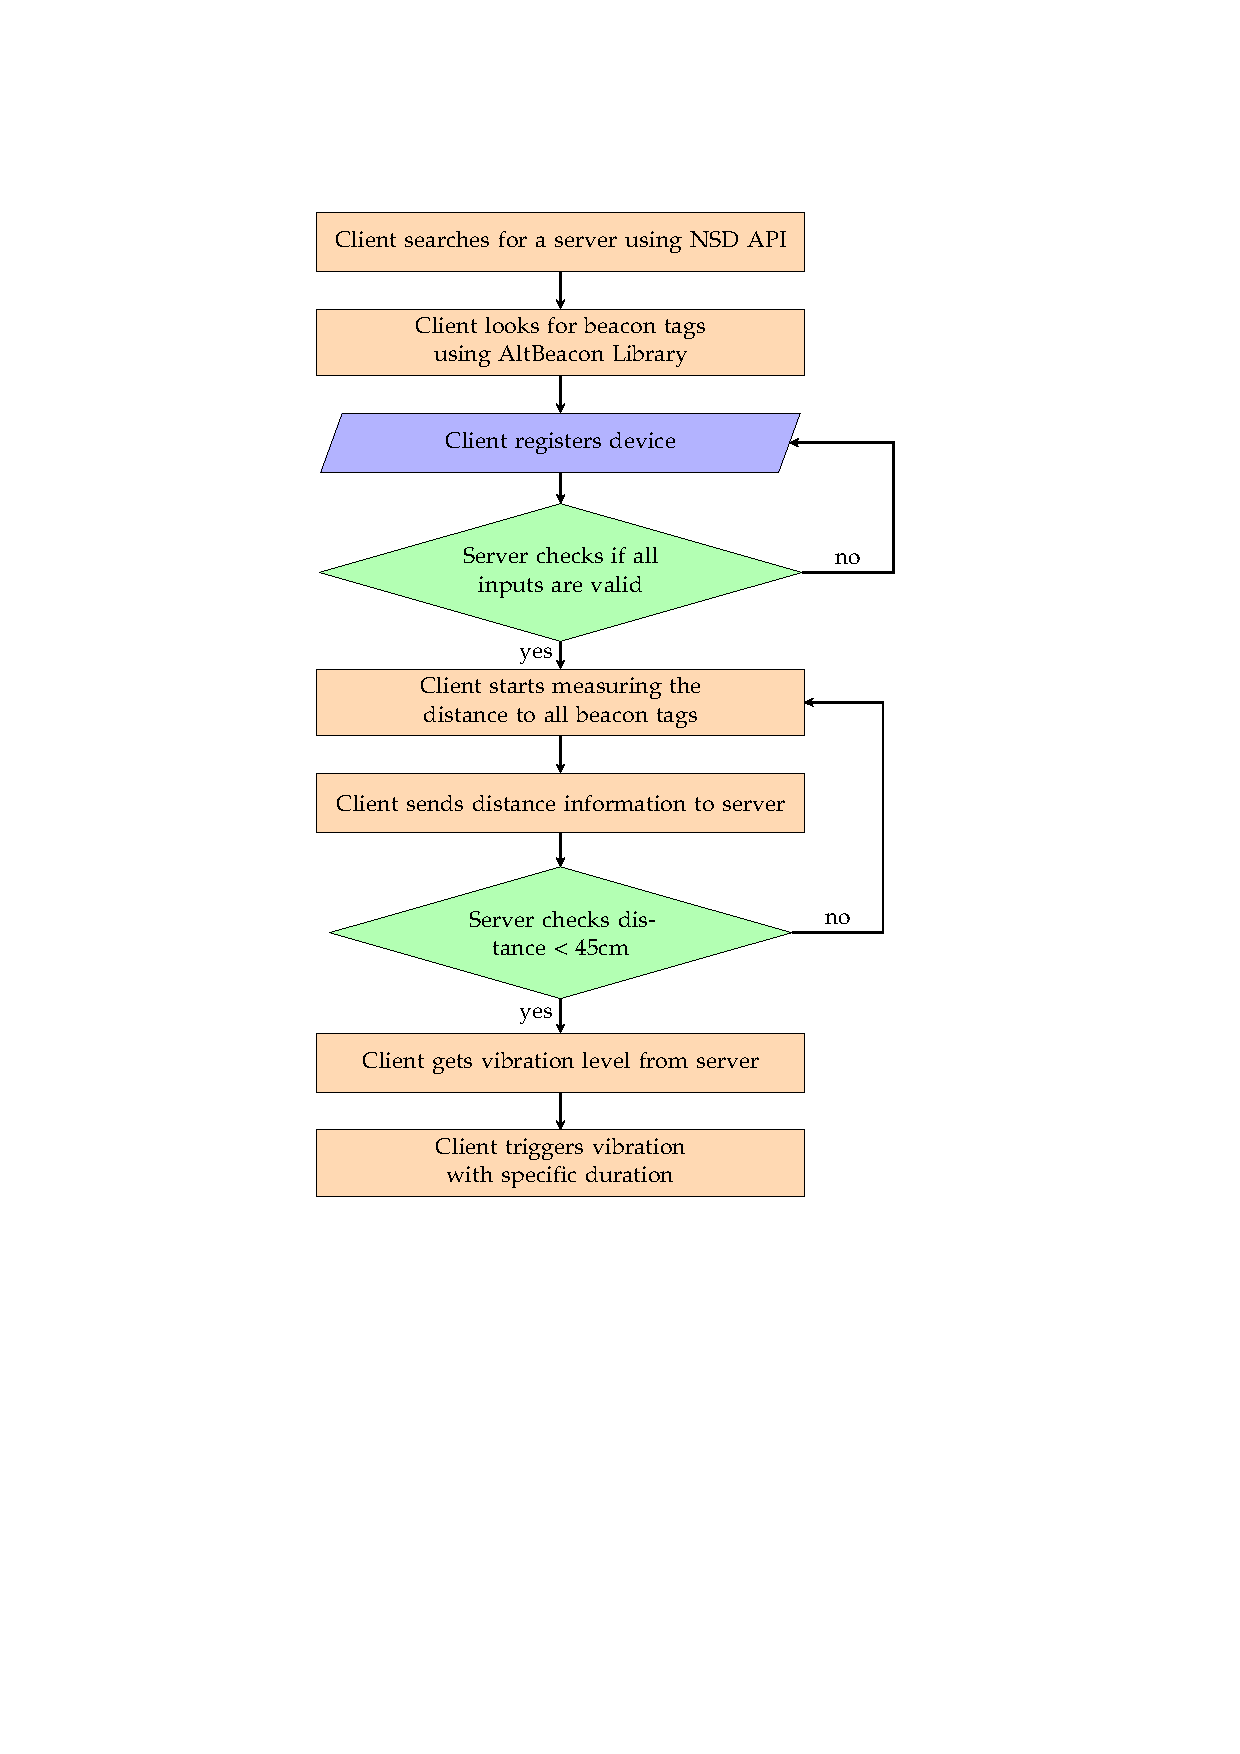
\includegraphics[scale=0.75]{WorkflowM-m.pdf}
%    \caption{The interaction between two phones and a server with the libraries and APIs that it is using.}
%    \label{fig:Stat12}
%\end{figure}
